% !TeX root = ../main.tex
% Add the above to each chapter to make compiling the PDF easier in some editors.

\chapter{eSIM Concept}\label{chapter:eSIMArch}
This chapter will give an overview of the two eSIM concepts for M2M and Consumer use cases. It will start with an introduction to (e)SIM cards, present shared objects and structures between the two and highlight the components and procedures of each architecture. In this section, the processes are only touched on superficially to enable the reader to place them in the overall context. The later chapter \ref{chapter:secAnalysis} "Security Analysis of eSIM" describes and analyzes the individual protocols and security mechanisms in more detail. The information for the M2M section is taken from the version 4.2 of SGP.01 \parencite{SGP:01} and version 4.2.1 of SGP.02 \parencite{SGP:02}. The description of the Consumer Architecture is relating to version 2.4 of SGP.21 \parencite{SGP:21} and SGP.22 \parencite{SGP:22}. A later version of SGP.21 (v3.0) has already been released at the time of writing, but not the corresponding technical specification. Therefore, a detailed analysis is not possible on the newest specification. However, a comparison will be made in the \ref{chapter:discussion}th section of this thesis.

%In this chapter, a brief overview of  the eSIM concept is given. What exactly does a SIM do, how does eSIM differ/evolve from this, and what is eSIM supposed to do?
%What does M2M and Consumer mean in regard to eSIM? Who uses/is supposed to use it. Are there similarities?

%The sub-chapters should describe the architecture and components of the eSIM, both for M2M and Consumer.
%The description relates to v4.2 (M2M) and v2.4 (Consumer). 
%Additionally, the process to download or provision a new profile to an eUICC is described.

%What is an (e)SIM exactly?

\section{SIM and eSIM}

A Subscriber Identity Module (SIM) Card is a type of Universal Integrated Circuit Card (UICC) introduced in the 1990s. It has since played a fundamental role in mobile telecommunications because the SIM main function is to act as a secure element to store a profile containing the secrets for secure and authenticated access to the mobile network. SIM cards today are issued by a specific mobile network operator (\acrshort{MNO}). The end user negotiates a contract with the MNO and receives a personalized SIM card, containing the subscription data and network access keys (\acrshort{NAA}). After inserting the SIM into the device, communication over the operators network should be enabled.

Each SIM chip is uniquely identified by its Integrated Circuit Card Identifier (ICCID), a number up to 20 digits long. This number will always remain the same, even if any information on the SIM is rewritten. To identify the subscriber in the wireless world (i.e. the con tract made between end user and MNO) and his home network, another 15 digit number called IMSI (International Mobile Subscriber Identity) is used. The IMSI consists of a 3-digit Mobile Country Code (MCC), 2-3 digits Mobile Network Code (MNC) and the remaining digits for a sequential serial number (MSIN).

\begin{figure}[ht]
    \centering
    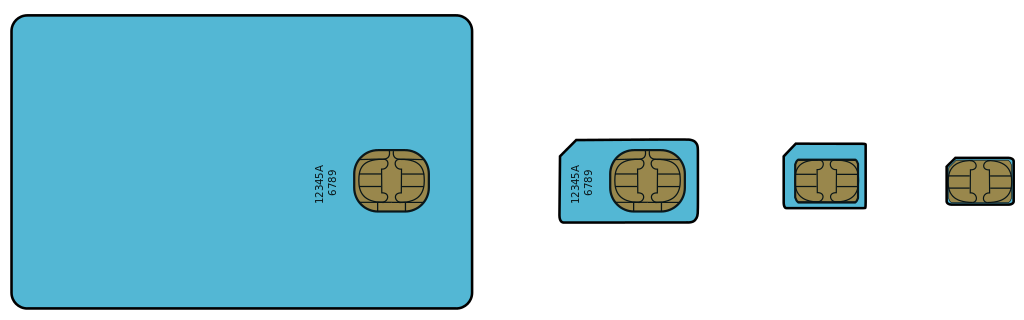
\includegraphics[width=0.75\textwidth]{pictures/sim_form_factors.png}
    \caption{SIM Form Factors: Full Size (1FF), Mini (2FF), Micro (3FF), Nano (4FF) \parencite{pic:SIMFormfactor}}
    \label{fig:sim-formfactors}
\end{figure}

SIM Cards can come in different form-factors, as seen in Figure \ref{fig:sim-formfactors}. The first SIM card was as big as credit cards are today (1FF). Since then, mobile or smartphones may have varied in sizes, but the number and size of internal components have increased, which results in the SIM cards needing to shrink over time, up to 4FF, which only measures 12.3 x 8.8 mm. Smaller layouts are not possible with regular SIM cards because of the standardized contact arrangement and usability. Embedding the chip into the device is the next logical step, since this allows for smaller footprints. At the same time, however, this brings an already existing problem with the SIM into even sharper focus: once the card is personalized by the MNO, it is not possible to change the stored credentials \parencite{Meyer:eSIMOverview}. If the user wants to switch to a different network operator, the SIM has to be physically replaced - which is obviously not possible with a soldered one. 

Thus, in 2018 the GSMA has released a new standard to tackle this problem with an embedded SIM (eSIM). The intention is, that it is now possible to remotely provision, enable, disable or delete the profile stored on the embedded UICC (eUICC) without changing the hardware. Once a profile is installed and enabled on the eUICC, it should function exactly as a traditional SIM and therefore be compatible with any existing mobile infrastructure. The standard packaging of eSIM is "MFF2", a solderable chip with dimensions of 6 x 5 mm, three times smaller than 4FF - but the contained technology can come in any form-factor \cite{1ot:SIMtypes}.

To enable the remote SIM provisioning (\acrshort{RSP}), five different actors can be defined \parencite{Gerpott:eSIM, Meyer:eSIMOverview}:
\begin{itemize}
    \item eUICC Manufacturer (EUM): The eSIM vendor fabricates and personalizes eUICCs by creating individual cryptographic keys and certificates. The confidential information is securely stored on the eICC and public information alongside the eUICCs characteristics are contained in an eUICC Information Set (\acrshort{EIS}).
    \item Subscriber: This could be the device manufacturer, an end user or a virtual entity. The subscriber manages his devices and attached eUICCs, which could be only one when it's a consumer with their personal mobile phone, or several thousands for an industrial customer. Subscribers are also the ones initiating profile management operations by contracting with operators.
    \item Device with eUICC: The device and eUICC are the endpoint of any remote profile management operation. The eUICC securely stores the profile package and any other relevant application, while the device takes advantage of the eUICCs capabilities to connect to the mobile network.
    \item Mobile Network Operator (MNO): The MNO runs telecommunication networks, is the owner of network access profiles and may also be a device reseller. A MNO may also directly interact with a profile installed on an eUICC to change any contained metadata.
    \item Provisioning Servers: These make up the actual RSP architecture. They are interacting with MNOs, Subscribers, eUICCs and with each other to generate a profile and install it on the target eUICC. They will be described in more depth later in this chapter.
\end{itemize}



\begin{figure}[ht]
    \centering
    \fontsize{8}{10}\selectfont
    \includesvg[width=0.7\textwidth]{pictures/profile_lifecycle}
    \caption{Profile Life-cycle}
    \label{fig:prof_lifecycle}
\end{figure}

One eSIM can hold multiple profiles, but with the current specification, only one profile may be active at a time. A regular profile consists of Network Access Keys (NAAs), Profile Policy Rules (POL), Operator OTA Keys (MNO-SD) and other applets or metadata depending on the profile type. Once created, the profile is stored on the SM-DP Server and ready for download. Every profile starts in a "disabled" state on the eUICC, but usually it will be enabled shortly after the installation. In the operational phase (see Figure \ref{fig:prof_lifecycle}), the NAAs are used to access the mobile network, and the operator can interact with his profile to change metadata (e.g. the displayed profile name) via his OTA keys. 

For eSIMs, two identifiers are mainly used in contrast to their usage with "regular" SIMs:
\begin{itemize}
    \item ICCID: The Integrated Circuit Card Identifier is now used to uniquely identify a profile in an eUICC instead of identifying the SIM Card. Length and format are identical as previously.
    \item EID: The eUICC Identifier is the replacement for the ICCID and works similar to a MAC-Address. It is stored inside the ECASD and is unique for every eSIM. There are two different formats defined, the IIN and EIN based format. They differ, as the Issuer Identification Number (IIN) has a fixed length of 8 digits, while the EUM Identification Number (EIN) may be longer. In the IIN-Format, the EID is exactly 32 digits long, with the first 18 digits identifying the card issuer. This is followed by 12 digits for the unique identification of the eUICC and 2 digits for a verifiable checksum.
\end{itemize}

Individual profiles can be assigned special attributes so that there is always exactly one "fallback" profile on the eSIM and optionally also an "emergency" and/or "test" profile. Through the POL it is also possible to specify that the profile must not be deactivated, or that it must be deleted if it is disabled. At the end of its life, the profile and all associated traces must be deleted from the eUICC and online registers must be updated accordingly.

The eSIM as described in the GSMA standard caters two different solutions, one for consumers \parencite{SGP:21} and one for machine to machine (M2M) \parencite{SGP:01} type communication. In the consumer-spec, the user can "pull" a new profile from a trusted server, where as in the M2M-spec, a "push" type system is used to provide a fleet of devices with new profiles without requiring additional end-user interaction. The key-points needed for profile provisioning of the two architectures will be explained in the following two sections.


\section{M2M}
%What is M2M, why does it need a eSIM?
%What does eSIM M2M do? Broad description of use-cases
Machine to Machine (M2M) devices are ubiquitous and communicate without human intervention. They have diverse applications, ranging from smart (e.g., smart-meters or -cars) and medical devices, to plant-production and vending machines, for instance. A growing number of devices communicate over cellular networks, relying on infrastructures owned by Mobile Network Operators, who restrict network access to subscribers. The secret keys needed to access the network are stored in a SIM-Card. 

However, as it is not feasible and often not possible to manually switch the SIM of some hundreds of devices once the network subscription changes, a mechanism is needed to remotely provision the profiles. The M2M eSIM allows this mechanism via multiple components, as described in the following sections. 

\subsection{Components}
\begin{figure}[ht]
    \centering
    \includesvg[width=0.9\textwidth]{pictures/m2m_architecture}
    \caption{M2M Architecture}
    \label{fig:m2m_arch}
\end{figure}
The infrastructure of the M2M eSIM consists of several nodes who interact with each other, as shown in Figure \ref{fig:m2m_arch}. The actors, as defined previously, still exist and the provisioning server architecture is split into two Subscription Managers: One for Data Preparation (SM-DP) and one for Secure Routing (SM-SR). The provisioning service should not require end-user interaction, follow a server-driven (push) model and impose only minimal further requirements on the - often already resource constrained - device. The security and authenticity of all operations in the M2M system relies on a mixture of symmetric keys (between SM-SR and eUICC) and Public Key Certificates issued by the GSMA CI.

In the next subsections, the tasks and functionality of the nodes mainly used for profile provisioning (eUICC, SM-SR and SM-DP) are explained, while the registration and profile provisioning process itself is highlighted later in chapter \ref{sec:M2MProfile}.

\subsubsection{eUICC}
The embedded Universal Integrated Circuit Card (\acrshort{eUICC}, Orange Box in Figure \ref{fig:m2m_arch}) is a discrete or integrated, tamper resistant, hard- and software component conforming to GlobalPlatform UICC Standards. It is - in general - non-removable and must be capable of hosting applications and cryptographic data \parencite{SGP:01}. The eSIM must at all times contain at least one operational profile with the "fallback" attribute set. While the eUICC can contain other multi-purpose applets, three security domains are accurately defined and relevant to conform with the eSIM Architecture:

\begin{itemize}
        \item ECASD: The "eUICC Certificate Authority Security Domain" is responsible for certificate and key management on the Secure Element. It is configured by the EUM during manufacturing and can never be disabled or deleted thereafter. It contains the non-modifiable eUICC asymmetric key-pair, associated certificate and GSMA CI public key. The ECASD is therefore closely collaborating with the ISD-R, as it is required for any certificate verification and key-establishment operation.
        \item ISD-R: The "Issuer Security Domain Root" executes platform management commands sent by the SM-SR. It is also created at manufacturing, cannot be deleted or disabled and is personalized with a symmetric AES-128 key. This key is bound to the responsible SM-SR and used to encrypt the communication among them. but could be replaced when the SM-SR is changed. The ISD-R can create and destroy ISD-Ps on the eUICC, but must not be allowed to modify or create any other security domain on the card.
        \item ISD-P: The "ISD Profile" has a similar life-cycle to the profile and is the only on-card security domain where multiple instances are allowed and which can be created and torn down at any time. One ISD-P holds exactly one profile and provides a key-establishment protocol for the SM-DP to encrypt the profile during download. Once the profile is installed on the eUICC, the ISD-P and profile create a union, whose state is managed by the ISD-P.
\end{itemize}

To be able to communicate with the remote provisioning servers, the eUICC must support at least sending and receiving SMS, and an IP-based application protocol, specifically either HTTPS or the Card Application Toolkit Transport Protocol (\acrshort{CATTP}), or both. A visualization of the protocol stack for an eUICC is given in Figure \ref{fig:prot_stack}.
\begin{figure}[ht]
    \centering
    \fontsize{7.7}{9.3}\selectfont
    \includesvg[width=0.7\textwidth]{pictures/protocol_stack}
    \caption{UICC Protocol Stack}
    \label{fig:prot_stack}
\end{figure}
The eUICC is not capable of handling an entire IP-Stack, but the management commands must be sent over a regular internet connection. Therefore, the server utilizes the correct application protocol, encrypts it appropriately (TLS or SCP80), and sends it to the M2M device. The device handles the IP-Stack and unwraps it up to the transport layer. Through a set of standardized smart-card protocols (Bearer Independent Protocol) and commands, the data is sent to the eUICC. The eUICC is also the encryption end-point, since only the ISD-R or ISD-P have the corresponding keys. 


\subsubsection{SM-SR}
In the M2M specification, all management operations on the eUICC are initiated by the "Subscription Manager - Secure Routing" (SM-SR). An SM-SR has a 1-n relationship to its eSIMs and uses individual symmetric keys to establish a secure and authenticated channel with them. This server is certified by the GSMA and may take instructions from other actors in the system (MNO, SM-DP, EUM). All of these interfaces are secured via TLS. The SM-SR acts as an intermediary between the SM-DP and eUICC during the profile download. It is also possible to move eSIMs from one SM-SR to another by generating new key material during the handover. 

The first SM-SR however requires a registration process through the EUM. The EUM produces the eUICC and personalizes the ISD-R and ECASD by generating and flashing key material. For each eUICC, an individual certificate is generated and signed by the EUM's certificate authority, which is accredited by the GSMA. The eUICCs public key certificate and symmetric management key is provided to the SM-SR inside an "eUICC Information Set" (EIS). The SM-SR must always protect this EIS, as any other organization with access to the symmetric key can also manage the target eSIM.  

\subsubsection{SM-DP}
The "Subscription Manager - Data Preparation" (SM-DP) is in turn responsible for generating and providing profile data. It receives a profile description from an operator and creates a generic profile accordingly. This bare-bone profile is then personalized for the targeted eUICC by incorporating the individual network access keys and secures the data with Profile Management Credentials of the eSIM.
The SM-DP always acts on behalf of the operator and may forward any management requests to the responsible SM-SR. One SM-DP is however not bound to one SM-SR or eUICC, that is why it must always authenticate itself before performing any operation. 

\subsection{Profile Provisioning Process} \label{sec:M2MProfile}
This section will give an overview of the profile download and installation process as described in the M2M specification. Security mechanisms and protocols are only briefly mentioned, a more detailed description will be given in the Security Analysis section (Chapter \ref{chapter:secAnalysis}). However, this high-level overview will provide useful guidance for the reader, as the entire provisioning process is somewhat tedious. 

\begin{figure}[ht]
    \centering
    \fontsize{7.7}{9.3}\selectfont
    \includesvg[width=0.8\textwidth]{pictures/m2m_high_level_download}
    \caption{M2M Profile Download}
    \label{fig:m2m_download}
\end{figure}

The eUICC must first be registered at its SM-SR and the device owner wants to download a new profile onto his eSIMs. Through a subscription process, the device owner orders the profiles from the operator and provides a range of EIDs. The MNO then contacts a selected SM-DP to first create generic profiles for this order and later personalize the profiles with individual network access keys. 

As a second operation, the operator initiates to profile download. The SM-DP and SM-SR mutually authenticate each other with their respective certificates. Any further communication should be secured via TLS. To be able to authenticate the eUICC later on, the SM-DP also requests the EIS associated to the eSIM from the SM-SR. Alongside its X509-certificate, this EIS also contains information about the already installed profiles, which the SM-DP needs to determine, if enough memory space is left on the eUICC to install a new profile. If all checks pass, the SM-DP forwards the installation request to the SM-SR.

Now, the SM-SR sends an encrypted SMS to the eUICC to trigger a remote management session. Since only the SM-SR can have the symmetric key to encrypt this SMS, the eUICC trusts its authenticity. However, depending on the used transport protocol (HTTPS, \acrshort{CATTP} or SMS), the eUICC (in particular, the ISD-R) and SM-SR may perform a session key agreement protocol to secure any further communication. To be ready for the profile installation, the ISD-R then creates an empty ISD-P. With the SM-SR and ISD-R as intermediaries, the SM-DP and ISD-P authenticate each other and establish a new session key. The SM-DP uses the certificate received in the EIS to determine the eUICCs public key while the ECASD on the eUICC helps to validate the received SM-DP certificate. The profile is encrypted with this session key and pushed to the eSIM. Only the ISD-P can decrypt the profile data, so the SM-SR and ISD-R forward any APDUs. The ISD-P and profile is now in a disabled state, and all involved actors have received a notification about the successful installation.

Lastly, the profile must be enabled. This process involves only the SM-SR and eUICC, but is triggered by either the operator, SM-DP or M2M Service Provider. The SM-SR sends the profile enabling command to the eUICC, which reviews the current profile policy (POL). If POL allows, the current profile will be disabled and the requested one enabled. The device tries to attach to the network and sends a success-notification to the SM-SR. If no answer is received, the eUICC assumes no network connectivity and re-enables the old profile.

\section{Consumer}
SIM Cards today are predominantly used in an end-user environment. An individual contracts with an operator to activate the mobile network subscription of his personal device (mobile phone, tablet or even car). The service (and SIM card) is and should be controlled by the client, since he knows his needs and can tailor or switch the contract accordingly. Therefore, a profile in the eSIM architecture should also be manageable by the Consumer and follow a client driven (pull) model.

Additionally, the use-cases in the consumer world require a more sophisticated model: In the M2M Spec, a single provisioning method suffices, as all devices are supposed to be managed over the same, top-down interface. The simplest and most established option for a consumer is to download a new profile on his phone. But how is the device enabled to download a profile? Which server should be contacted and how can they authenticate each other to find the correct profile? The process becomes even more complex if the profile is not destined for a phone, but for the eSIM inside the user's smartwatch. Hence, the GSMA has built a second eSIM architecture for Consumers, which will be described in the next sections.

\subsection{Components}
Many of the components in the Consumer specification \parencite{SGP:21} are re-designed versions of the M2M architecture. The provisioning servers are now split into one for the download process (SM-DP+) and one for discovery services (SM-DS). Since the End-User wants to directly interact with the eSIM of his personal device, a Local Profile Assistant (\acrshort{LPA}) is needed instead of a remote service. This also ensures, that any management process starts only after the user has consented to it.
The security and authenticity of all operations in the Consumer system relies solely on Public Key Certificates issued by the GSMA CI.

In the next subsections, these components (see Figure \ref{fig:con_arch}) will be listed and explained. However, since these are in some cases very similar to the M2M version, we refer to the previous description in each case.

\begin{figure}[ht]
    \centering
    \includesvg[width=0.9\textwidth]{pictures/consumer_architecture}
    %\includegraphics[width=0.75\textwidth]{pictures/M2M_arch.png}
    \caption{Consumer Architecture}
    \label{fig:con_arch}
\end{figure}

\subsubsection{eUICC}
The Consumer eUICC's security domains (ISD-R, ISD-P and ECASD) are identical to the ones defined in the M2M specification. The eSIM may now be removable from the device and it is allowed for the eUICC to be provisioned with zero installed profiles. Without any mobile network connection, the first (or any other) profile download should be possible over any device interface (e.g. Wi-Fi, Bluetooth, etc.). Additionally it can be expected, that the ownership of the secure element changes more often during its lifetime. Therefore, a memory reset must be supported to delete any user information.

\acrshort{CATTP}, as mentioned in Figure \ref{fig:prot_stack}, is not used on a Consumer eSIM. The only required application protocol is \acrshort{HTTPS}. In this case, though, the ISD-R does not contain a symmetric key, since all operations require a key-establishment protocol based on the eUICCs certificate.

\subsubsection{LPA}
The Local Profile Assistant manages profile operations and interacts with the eUICC. It is often an application on the host-device (LPAd) but can also be running directly on the secure element (LPAe). Since the location of the LPA must not matter for its functionality, in the remainder of this thesis both options will be referred to as \acrshort{LPA} only.

An LPA consists of up to three services, each managing an interface to one external actor and to the ISD-R:
\begin{itemize}
    \item LPD: The Local Profile Download Service is the heart of the LPA and interacts with SM-DP+ to download a new profile. It plays a proxy role in the provisioning process, as it downloads the bound profile package in a single transaction from the SM-DP+, segments it for the eUICC and transfers these segments sequentially.
    \item LDS: Event records issued by the SM-DS are received by the Local Discovery Service. It is responsible for retrieving the Root-SM-DS Address from the eUICC, building a secured connection to the SM-DS, polling new events and notifying the LPD over any pending management operation.
    \item LUI: Interactions with the end-user are handled by the Local User Interface. Parsing an Activation Code, listing profiles, local profile management and confirming user consent for any operation is done by the LUI. This LPA service can also run on a companion device (e.g. Smartwatch with eSIM performs profile download over mobile phone), since the companion device may have better user interaction capabilities. 
\end{itemize}

\subsubsection{SM-DP+}
The SM-DP+ combines the functionalities of the SM-DP and SM-SR of the M2M Specification. It builds the profile according to the operator's specification (Unprotected Profile Package), encrypt-then-mac's it with profile protections keys (Protected Profile Package) and generates a "Bound Profile Package", which are package segments and personalized to a specific eUICC. Protected or Bound Profile Packages can be stored on the SM-DP+ until they need to be downloaded. 

Additionally, the SM-DP+ can register and query events at the SM-DS for a specific eUICC.

\subsubsection{SM-DS}
If an SM-DP+ wishes to communicate with an eUICC, it can register an event for this specific eUICC at the appropriate "Subscription Manager - Discovery Service". The SM-DS does not know the content of the event, as they are purely managed by the SM-DP+. The target eSIM must poll for new events at their root SM-DS. SM-DS can also internally cascade events, if the registration by an SM-DP+ did not occur on the root SM-DS responsible for the requested EID. 

An event is often needed, when an update of an already downloaded profile is required, or in first-boot scenarios: A mobile phone is sold to an end-user by an operator. This phone's eSIM is already personalized by the operator and will poll the SM-DS as soon as it boots for the first time. The SM-DS then provides information on how and where to download the network profile. This simplifies the provisioning process for the end-user, as all that is required from him is the consent to download the profile.

\subsection{Activation Code}
A profile download can be initiated in three ways: Either by retrieving an event from the SM-DS, contacting the default SM-DP+ and querying for a new profile, or by entering an activation code on the LUI.
This AC often comes in the form of a Quick Response (QR) Code, but must also be able to be typed in by hand for devices without any camera. Thus, the data element is limited to a maximum length of 255 characters. 

The mandatory and optional content of the activation code, can be seen in Table \ref{tab:ConAC}:

\begin{table}[htpb]
    \caption[Activation Code]{Activation Code}\label{tab:ConAC}
    \centering
    \begin{tabular}{m{3cm}|m{6cm}|c|m{3cm}}
         Name & Description & MOC & Example Value\\ \hline
         AC Format & Format of this activation code, only "1" & M & 1 \\ \hline
         Delimiter & & M & \$ \\ \hline
         SM-DP+ Address & FQDN of the SM-DP+ & M & SMDP.GSMA.COM \\ \hline
         Delimiter & & M & \$ \\ \hline
         AC Token & Matching-ID for Profile Download & M & 04386-AGYFT-A74Y8-3F815 \\ \hline
         Delimiter & & C & \$ \\ \hline
         SM-DP+ OID & SM-DP+ OID as in Certificate & O & 1.3.6.1.4.1.31746 \\ \hline
         Delimiter & & C & \$ \\ \hline
         Confirmation Code Required Flag & If a confirmation code is required, it must be 1, otherwise missing. & O & 1
    \end{tabular}
\end{table}
The only mandatory data elements are the format identifier, SM-DP+ Address and the activation code (AC) token. The AC Token is generated by either the operator or SM-DP+ and is giving the SM-DP+ information to find the correct context for the specific management order of the requesting eUICC, once the provided Fully Qualified Domain Name (FQDN) of the SM-DP+ has been resolved. 

The SM-DP+ Object Identifier (OID) is already optional, but if it is provided, it has to match the OID in the certificate received during the mutual authentication of SM-DP+ and eUICC.
If a Confirmation Code is required for the profile download, the flag must be set in the activation code. The CC is a second-factor authentication for the SM-DP+, such that the correct profile has been requested by the correct end-user. It must not be contained in the activation code, but given to the end user in a separate way. The user types it into the LPA, which provides a hash for confirmation to the SM-DP+.
It is also possible, that the "Confirmation Code Required Flag" is set, but not the SM-DP+ OID. Then, the field in the AC is of zero-length, but separated by two delimiters (i.e. "[...]\$\$1").


\subsection{Profile Provisioning Process}
Downloading and installing a profile in the consumer architecture is different, as every action is initiated by the end-user and all parties must authenticate each other before communication due to the public key infrastructure.

\begin{figure}[ht]
    \centering
    \fontsize{7.7}{9.3}\selectfont
    \includesvg[width=0.95\textwidth]{pictures/consumer_high_level_download}
    \caption{Consumer Profile Download}
    \label{fig:consumer_download}
\end{figure}

The Download Initiation Phase starts with the End User subscribing to a contract with the MNO. Based on the information provided by the user and device capabilities, the MNO orders a profile at his SM-DP+, which creates a Protected Profile Package, meaning the data is already encrypted with session keys only known to the SM-DP+. The Figure \ref{fig:consumer_download} and the remaining section assumes the use of an Activation Code as provisioning method. Therefore, a unique Matching-ID (a combination of alphanumeric characters) is sent to the MNO along with information on the created profile (e.g. ICCID). The Operator generates the Activation Code and supplies it to the consumer.

By entering the Activation Code into the LPA, the Common Mutual Authentication Procedure is stated. It is a device initiated process, where the LPA first asks the eUICC for its info and a random challenge. After establishing an HTTPS session with the SM-DP+ using Server Authentication Mode, the eUICC and SM-DP+ authenticate each other by sending and verifying a set of challenges, signatures and information about the profile download (i.e. the Matching-ID). As a last step of this phase, the profile metadata is sent to the LPA.

Lastly, the profile download and installation phase takes place. The LPA checks the received profile metadata and allowance of policies (PPR1/PPR2) and presents the user a download confirmation request. A new ISD-P is created and an Elliptic Curve Key Agreement (ECKA) is performed with the SM-DP+ to personalize the ISD-P. This one-time session key is used by the SM-DP+ to further encrypt the PPP and make it a Bound Profile Package (BPP). The LPA downloads the BPP in a single transaction, segments it into smaller APDUs and transports the segments to the eUICC. After re-arranging the profile package, decrypting and installing it, the ISD-P is now ready to be enabled. The end-user can do so through his LPA.